\documentclass[answers]{exam}
\usepackage[utf8]{inputenc}

\usepackage[dvipsnames]{xcolor}
\usepackage{amsmath}
\usepackage{amsfonts}
\usepackage{amsthm}
\usepackage{microtype}
\usepackage{siunitx}
\DeclareSIUnit\year{yr}
\usepackage{pgfplots}
\usepackage{graphicx}
\usepackage{sidecap}
\sidecaptionvpos{figure}{c}
\usepackage{float}
\usepackage{gensymb}
\usepackage{tkz-euclide}
\usetkzobj{all}
\usepackage{commath}
\usepackage{hyperref}
\usepackage{enumitem}
\usepackage{wasysym}

\renewcommand*{\thefootnote}{\fnsymbol{footnote}}

\newtheorem*{thm}{Theorem}
\newtheorem*{iden}{Identity}
\newtheorem*{lemma}{Lemma}
\theoremstyle{definition}
\newtheorem*{defn}{Definition}
\newtheorem*{ex}{Example}

% russian integral
\usepackage{scalerel}
\DeclareMathOperator*{\rint}{\scalerel*{\rotatebox{17}{$\!\int\!$}}{\int}}

% \qformat{Question \thequestion: \thequestiontitle\hfill}

\begin{document}

\section*{NCEA Level 3 Physics (Modern Physics)}
Heinrich Hertz was a German physicist who was the first to conclusively prove
the existence of electro-magnetic waves (light). In 1887, he observed an interesting
phenomenon: when light strikes a metal surface, electrons are emitted. This is known
as the \textit{photoelectric effect}.

\subsection*{The photoelectric effect}
When UV light falls on a sheet of metal, its energy is absorbed and some is transferred
to electrons which are ejected as fast-moving particles (photoelectrons). A certain amount
of energy must be transferred to an electron before it can be emitted; this amount is
dependent on the type of metal and is known as the \textit{work function} $ \phi $ of the metal.
This energy is quite small in absolute terms, and can easily be provided by electro-magnetic waves.
However, some observations surrounding the photoelectric effect cannot be explained by treating
light as a wave, and seem to suggest that light in fact acts as a particle!

\begin{center}
\begin{tabular}{|p{0.4\linewidth}|p{0.4\linewidth}|}
  \hline
  \textbf{Predicted by the wave theory} & \textbf{Observed phenomena}\\\hline
  A brighter light would cause electrons to have greater kinetic energy when released. &
  Brighter light caused \textbf{more} electrons of the \textbf{same} kinetic energy to be released.\\\hline
  If a dim light were used, electrons would need to accumulate energy to overcome the work function and so would not be emitted instantaneously. &
  When UV light was used, even the faintest light caused instant electron emission.\\\hline
  The frequency of light would not cause any change in observations. &
  A higher frequency of light caused electrons to have a higher kinetic energy. Below a certain frequency,
  no electrons were emitted.\\\hline
\end{tabular}
\end{center}

On the other hand, from experiments like Young's double-slit experiment, we know that
light can sometimes act as a wave!

\begin{center}
  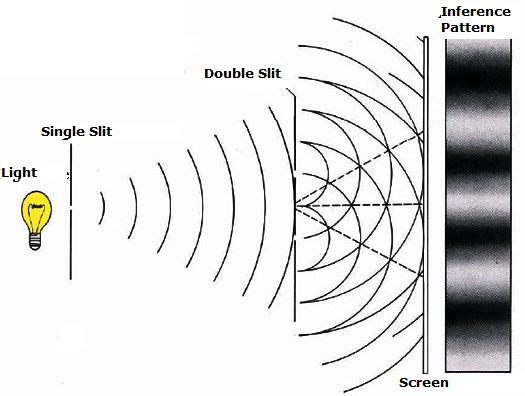
\includegraphics[width=0.5\textwidth]{doubleslit}
\end{center}

Albert Einstein, a German physicist, discussed the photoelectric effect in 1905 using the
idea of \textit{quantization} that was put forward by Max Plank. In essence, it was
proposed that electro-magnetic radiation comes in packets (quanta) of fixed size known
as \textit{photons}; the energy of an individual photon is directly proportional to the frequency of
light, with a constant of proportionality $ h \approx \SI{6.63e-34}{\joule\second} $ known
as \textit{Plank's constant}:
\begin{displaymath}
  E = hf.
\end{displaymath}

If we apply this to the photoelectric effect, we find that the energy of emitted photoelectrons
when light of frequency $ f $ is incident can be found (and recalling that $ \phi $ is the work
function of the metal).
\begin{displaymath}
  E = hf - \phi
\end{displaymath}

This allows us to calculate the \textit{critical frequency} of the metal --- the frequency $ f_0 $ which
is at the threshold of electron emission. If the frequency of incident light is less than $ f_0 $, no
light is emitted.
\begin{displaymath}
  0 = hf_0 - \phi \implies f_0 = \frac{\phi}{h}
\end{displaymath}

We can easily see the effects of the photoelectric effect by examining a photoelectric cell.
Recall that voltage is simply $ V = \frac{E}{q} $, and so $ E = qV $. Hence, if an electron
of charge $ e = \SI{1.6e-19}{\coulomb} $ is emitted from the cell then the cell must
lose an energy $ eV $; since energy is conserved, this energy must have gone to the emitted
electron.

\subsection*{Questions}
Useful data: $ c \approx \SI{2.99e8}{\metre\per\second} $, $ h \approx \SI{6.63e-34}{\joule\second} $,
$ e \approx \SI{1.6e-19}{\coulomb} $, $ \SI{1}{\electronvolt} \approx \SI{1.6e-19}{\joule} $

\begin{questions}
  \question The frequency of a photon of red light is \SI{4.57e14}{\hertz}. Calculate the energy of the photon.
  \question Calculate the energy of a photon of blue light with a wavelength of \SI{4.0e-7}{\metre\per\second}.
  \question Consider the following properties of light; which are better explained by a wave theory of light, and
            which by a particle theory?
    \begin{parts}
      \part Reflection
      \part Diffraction
      \part Interference
      \part The photoelectric effect
    \end{parts}
  \question A metal plate has a work function of $ \phi = \SI{5}{\electronvolt} $. If EM radiation
            with a wavelength of $ \lambda = \SI{2e-7}{m} $ falls on the plate, what is the energy
            of the emitted photons?
  \question In an experiment, blue light of frequency \SI{7e14}{\hertz} shines on a photoelectric
            cell and produces a cutoff voltage of \SI{1.63}{\volt}.
    \begin{parts}
      \part What is the energy of a photon of blue light?
      \part What is the maximum kinetic energy of the ejected electrons?
      \part What is the work function of the metal?
      \part What is the threshold frequency of the metal?
    \end{parts}
  \question What does the maximum kinetic energy of photoelectrons emitted from a particular
            metal depend on?
\end{questions}

\end{document}
